\chapter{Analisis Penyelesaian Masalah}
\label{chLanalisis}

Pada bab analisis masalah ini akan dibahas mengenai masalah yang akan diselesaikan beserta solusi yang ditawarkan. Selain itu bab ini juga akan membahas tentang contoh penyelesaian masalah dengan data yang skalanya lebih kecil. 

\section{Analisis Masalah}
\label{sec: Analisis Masalah}

Perkembangan dunia \web selama lima tahun terakhir sangat pesat. Pesatnya perkembangan dunia \web ini didukung oleh munculnya berbagai macam teknologi yang dapat digunakan untuk membuatnya. Banyaknya teknologi yang bermunculan ini tentunya digunakan untuk membuat \web semakin baik dari sisi performa maupun pengalaman pengguna \web. Perkembangan dari penggunaan teknologi ini kemudian dicatat oleh sebuah situs bernama \http. Situs ini menyediakan data yang mencatat berbagai matriks penilaian yang dapat mengukur baik maupun buruknya performa sebuah \web. Data yang disajikan tentunya tidak mudah untuk dimengerti oleh semua orang. 

Solusi yang ditawarkan untuk mempermudah pengguna data untuk mengerti data yang disajikan adalah dengan cara melakukan visualisasi yang sesuai. Visualisasi yang dilakukan juga dapat disesuaikan dengan kebutuhan dari pengguna sehingga visualisasi yang digunakan akan berupa visualisasi yang interaktif. Data yang sudah didapatkan kemudian diolah dengan menggunakan bahasa SQL untuk kemudian hasil \textit{query}. yang menghasilkan potongan data yang dibutuhkan, divisualisasikan ke dalam bentuk visualisasi yang dibutuhkan.

\section{Data Kecil}
\label{sec: datakecil}

Bagian ini akan berisi tentang penyiapan data kecil kemudian setelah itu akan dilanjutkan dengan melakukan pengolahan dan visualisasi dengan menggunakan data kecil.

\subsection{Penyiapan Data Kecil}
\label{subsec:penyiapan data kecil}

Data yang digunakan merupakan data \textit{sample} yang diberikan oleh \http yang berasal dari bagian \textit{public dataset} dan menggunakan tabel \textit{pages} seperti yang sudah dijelaskan pada \ref{subsec:pd}. Data yang digunakan berasal dari data yang sudah diperbaharui oleh \http. Data yang didapatkan adalah data dari tanggal 1 Februari 2024 sampai dengan 1 Februari 2025. Data yang digunakan akan lebih berfokus pada tanggal, teknologi, \textit{client}, dan url utama dari halaman \web, sehingga kolom dan baris lainnya tidak akan digunakan. Pengumpulan data dilakukan dengan melakukan \textit{query} dengan menggunakan \textit{Google Big Query}. Hasil dari \textit{query} tadi kemudian disimpan ke dalam format CSV (\textit{Comma Separated Value}). Salah satu query yang dapat digunakan untuk mengumpulkan data dapat dilihat pada Kode~\ref{kode:kumpuldatakecil}. Kode tersebut akan mengembalikan data yang berisi kolom \textit{date, client, root\_page}, dan \textit{technology} yang berasal dari tabel \textit{pages} dan data yang diambil berasal dari rentang waktu yang sudah disebutkan sebelumnya, namun data dibatasi 10.000.000 baris.

\begin{lstlisting}[language=SQL, caption=Kode untuk mengumpulkan data kecil, label=kode:kumpuldatakecil]

    SELECT date, client, t.technology, COUNT(t.technology),  
    FROM `httparchive.crawl.pages`, UNNEST(technologies) as t 
    WHERE date BETWEEN "2024-02-01" and "2025-02-01" limit 100000000
    
\end{lstlisting}

\subsection{Pengolahan Data Kecil}
\label{subsec:pengolahankecil}

Setelah data yang akan digunakan siap, hal selanjutnya adalah mengolah data tersebut. Pengolahan data ini akan menggunakan bahasa \textit{Python}. Dalam pengolahan ini perspektif yang dilihat adalah perkembangan sepuluh teknologi populer pada semua \textit{client}, perkembangan sepuluh teknologi populer untuk \textit{client} \mobile, dan perkembangan sepuluh teknologi untuk \textit{client} \desktop.

\subsubsection{Perkembangan Sepuluh Teknologi Populer}
\label{subsub: 10semua}
Hal pertama yang dilakukan adalah dengan memuat data \textit{sample}. Contoh dari data \textit{sample} yang dimuat dapat dilihat pada Tabel~\ref{tab:sample}. Data tersebut adalah hasil dari menjalankan kode berisikan tanggal diambilnya data, perangkat yang digunakan untuk mengambil data, url utama dari halaman \web yang dites, dan teknologi yang digunakan oleh halaman \web yang dites. Data tersebut didapatkan dengan menjalankan query pada potongan Kode~\ref{kode:kumpuldatakecil} 
\begin{table}[H]
    \centering
    \caption{Lima baris data \textit{sample}}
    \label{tab:sample}
    \begin{tabular}{|l|l|l|r|}
        \hline
        date & client & technology & jumlah \\ \hline
        2025-02-01 & desktop & Google Analytics & 12.370 \\ \hline
        2025-02-01 & mobile &  HSTS & 131\\ \hline
        2025-02-01 & mobile &  Klaviyo &  \\ \hline
        2025-02-01 & mobile & Gatsby & 268 \\ \hline
        2025-02-01 & mobile &  YouTube & 20.2669 \\ \hline
        ...&...&...&... \\ \hline
    \end{tabular}
\end{table}

Setelah itu kemudian data dikelompokkan berdasarkan teknologinya dengan menggunakan Kode~\verb|df_gb = df.groupby(["technology"]).sum('f0_')|. Contoh hasil dari pengelompokan data ini dapat dilihat pada Tabel~\ref{tab:gbsample}. Terlihat bahwa untuk tanggal yang sama ada berbagai teknologi dengan jumlah pemakaian dari berbagai halaman \web yang beragam. Data yang dikelompokkan juga berasal dari penggunaan teknologi untuk perangkat \mobile dan \desktop.
\begin{table}[H]
    \centering
    \caption{Contoh hasil pengelompokan data \textit{sample} berdasarkan teknologi yang digunakan}
    \label{tab:gbsample}
    \begin{tabular}{|l|l|r|}
        \hline
        date & technology & jumlah pemakaian \\ \hline
        2024-02-01 & Datadog & 4.591 \\ \hline
        2024-02-01 & Node.js & 14.794 \\ \hline
        2024-02-01 & Google Tag Manager & 124.814 \\ \hline
        2024-02-01 & Sendgrid & 12.152 \\ \hline
        2024-02-01 & Dojo & 2.087 \\ \hline
        ...&...&... \\ \hline
    \end{tabular}
\end{table}

Kemudian data yang sudah terkelompok diurutkan berdasarkan penggunaan paling banyak. Kode~\verb|df_sorted = df_gb.sort_values(by='f0_', ascending=False)| digunakan untuk mengurutkan data. Contoh hasil pengurutan ini dapat dilihat pada Tabel~\ref{tab:urutgbsample}. Terlihat bahwa teknologi yang paling banyak digunakan pada rentang waktu 1 Februari 2024 sampai 1 Februari 2025 adalah \textit{JQuery} dengan 4.464.436 halaman \web yang menggunakan teknologi ini untuk membangunnya.
\begin{table}[H]
    \centering
    \caption{Contoh data penggunaan teknologi yang sudah diurutkan berdasarkan pemakaian paling banyak}
    \label{tab:urutgbsample}
    \begin{tabular}{|l|r|}
        \hline
        technology & Jumlah Pemakaian \\ \hline
        jQuery & 4.464.436 \\ \hline
        Open Graph & 3.834.676 \\ \hline
        Google Analytics & 3.323.217 \\ \hline
        PHP & 3.294.059 \\ \hline
        Google Font API & 2.802.138 \\ \hline
        core-js & 2.573.059 \\ \hline
        ... & ... \\ \hline
    \end{tabular}
\end{table}

Setelah itu sepuluh teknologi yang paling banyak digunakan akan diambil. Kode yang digunakan untuk mencari sepuluh teknologi yang paling banyak digunakan adalah \verb|df_10 = df_sorted.head(10)|. Sepuluh teknologi dengan penggunaan paling banyak dapat dilihat pada tabel~\ref{tab:sepuluhsemua}. Terlihat bahwa dua teknologi dari \textit{jQuery} masuk sebagai sepuluh yang paling banyak dipakai di semua \textit{client} 

\begin{table}[H]
    \centering
    \caption{Sepuluh teknologi dengan jumlah penggunaan paling banyak untuk semua \textit{client}}
    \label{tab:sepuluhsemua}
    \begin{tabular}{|l|r|}
        \hline
        technology & Jumlah Pemakaian \\ \hline
        jQuery & 4.464.436 \\ \hline
        Open Graph & 3.834.676 \\ \hline
        Google Analytics & 3.323.217 \\ \hline
        PHP & 3.294.059 \\ \hline
        Google Font API & 2.802.138 \\ \hline
        core-js & 2.573.059 \\ \hline
        MySQL & 2.338.106 \\ \hline
        RSS & 2.236.824 \\ \hline
        WordPress & 2.112.285 \\ \hline
        jQuery Migrate & 2.041.754 \\ \hline
    \end{tabular}
\end{table}
Setelah sepuluh teknologi yang populer sudah didapatkan, hal selanjutnya yang dicari adalah penggunaan sepuluh teknologi tersebut dalam rentang waktu yang sudah ditentukan. Kode~\verb|df_pivot = df_baru.pivot(index="date", columns='technology', values='f0_')| digunakan untuk melakukan hal ini. Hasilnya kemudian divisualisasikan dan hasilnya dapat dilihat pada Gambar~\ref{fig:samplejumlah10}. Terlihat bahwa pola yang dihasilkan untuk semua teknologi sama, sehingga jumlah penggunaan ini akan dibagi dengan jumlah pemakaian semua teknologi di bulan yang sama.

\begin{figure}[H]
    \centering
    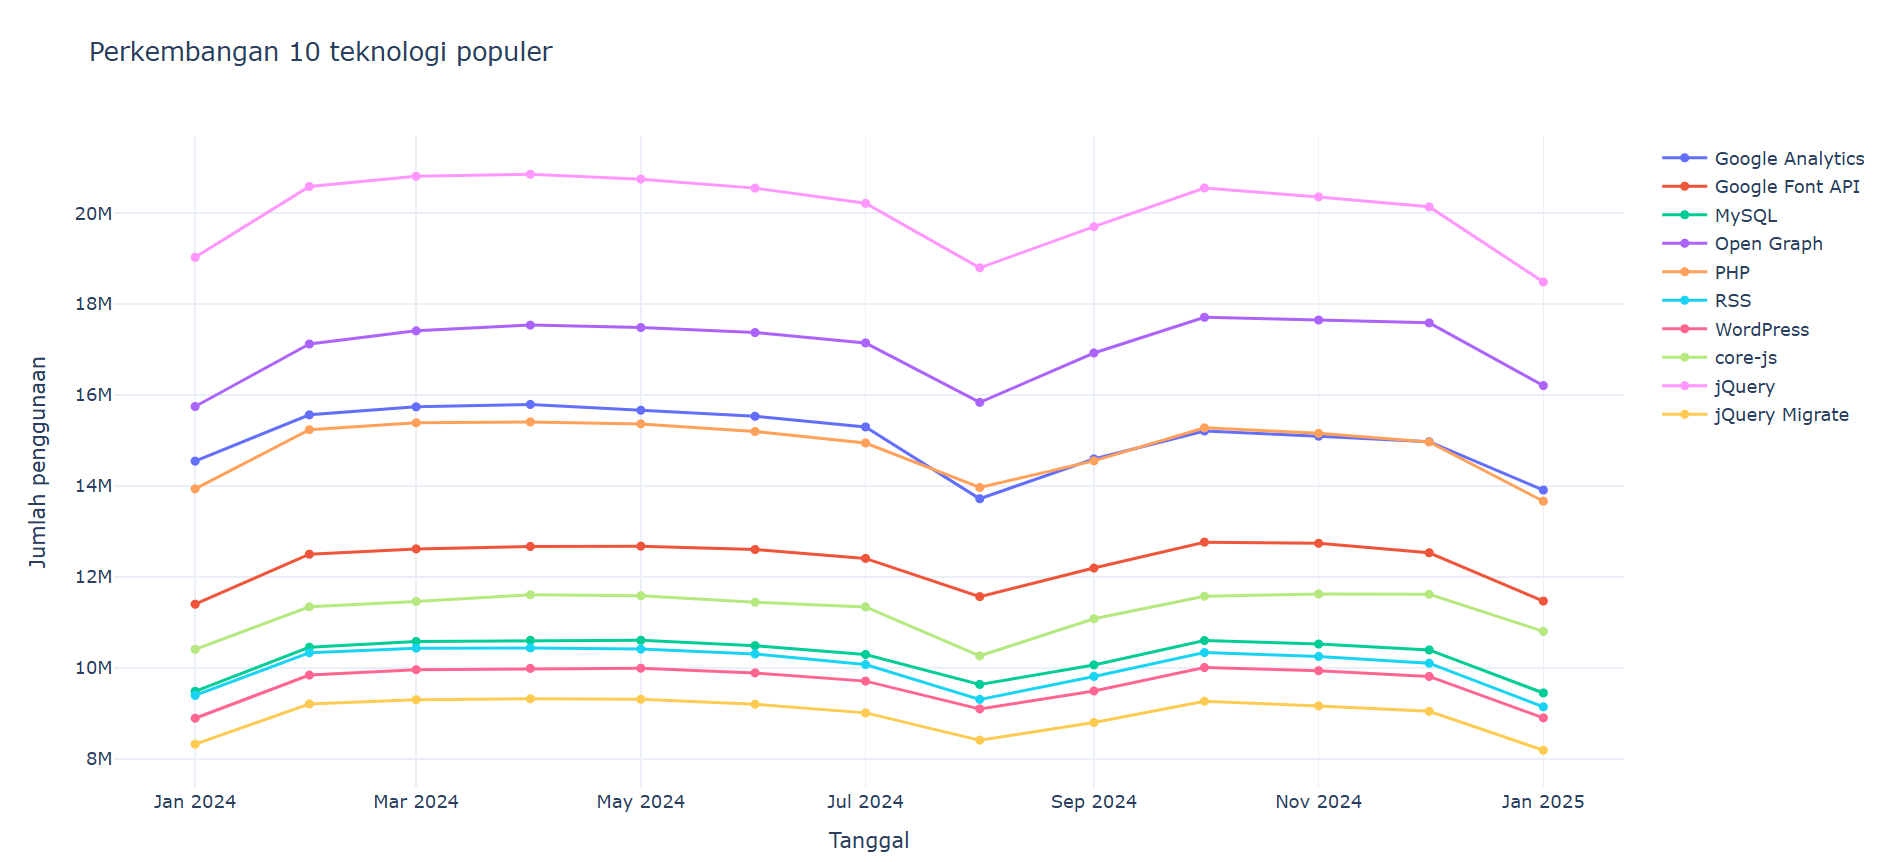
\includegraphics[width=0.7\linewidth]{Gambar/Perkembangan jumlah 10 teknologi populer.png}
    \caption{Perkembangan jumlah penggunaan sepuluh teknologi populer}
    \label{fig:samplejumlah10}
\end{figure}

Hal ini dilakukan agar lebih terlihat persentase pemakaiannya. Setelah itu hal yang dilakukan adalah memvisualisasikan data yang sudah didapatkan. Hasil visualisasinya dapat dilihat pada Gambar~\ref{fig:sample10}. Terlihat dari hasil visualisasinya bahwa untuk semua teknologi mengalami penurunan pemakaian pada tanggal 1 Agustus 2024. Selain itu semua teknologi terlihat memiliki perkembangan yang hampir mirip dan stabil.
\begin{figure}[H]
    \centering
    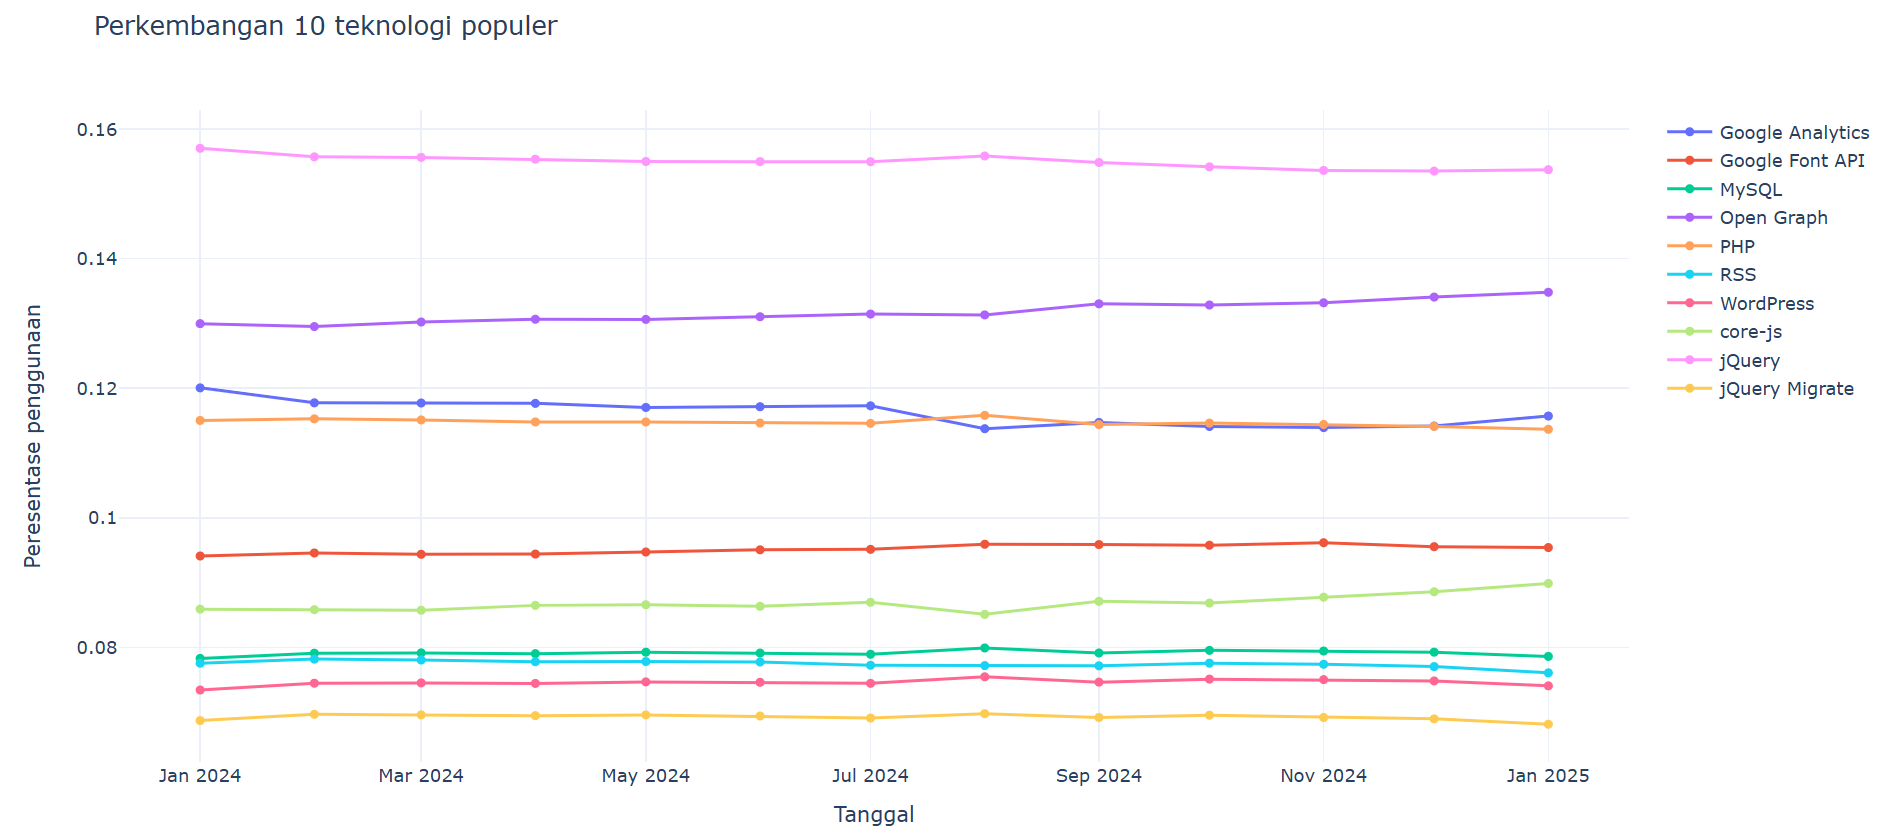
\includegraphics[width=0.7\linewidth]{Gambar/Perkembangan persentase.png}
    \caption{Perkembangan sepuluh teknologi populer berdasarkan persentase penggunaannya}
    \label{fig:sample10}
\end{figure}


\subsubsection{Perkembangan Sepuluh Teknologi pada \textit{Client} \mobile}
\label{subsub:10mobile}
Hal pertama yang dilakukan adalah dengan memuat data \textit{sample}. Contoh dari data \textit{sample} yang dimuat dapat dilihat pada Tabel~\ref{tab:sample}. Data tersebut berisikan tanggal diambilnya data, perangkat yang digunakan untuk mengambil data, url utama dari halaman \web yang dites, dan teknologi yang digunakan oleh halaman \web yang dites. Data tersebut didapatkan dengan menjalankan query pada potongan Kode~\ref{kode:kumpuldatakecil} 

Kemudian data yang memiliki \textit{client} \mobile diambil untuk dilakukan pengolahan lebih lanjut. Kode yang digunakan untuk memisahkan data ini adalah \verb|df_mobile = df[df['client'] == 'mobile]|. Kemudian data yang sudah dipisahkan dikelompokkan berdasarkan teknologi yang dipakai menggunakan kode \verb|df_mobile_gb = df_mobile.groupby(["technology"]).sum('f0_')|. Proses yang dilakukan masih sama seperti pada Bagian~\ref{subsub: 10semua} namun ada sedikit perbedaan pada sepuluh teknologi yang paling banyak digunakan seperti yang terlihat pada Tabel~\ref{tab:sepuluhmobile}. Pada \textit{client} \mobile terlihat bahwa teknologi PHP lebih banyak digunakan.
\begin{table}[H]
    \centering
    \caption{Sepuluh teknologi dengan jumlah penggunaan paling banyak untuk \textit{client} \mobile}
    \label{tab:sepuluhmobile}
    \begin{tabular}{|l|r|}
        \hline
        technology & Jumlah Pemakaian \\ \hline
        jQuery & 286.441.430 \\ \hline
        Open Graph & 245.369.426 \\ \hline
        PHP & 214.645.943 \\ \hline
        Google Analytics & 212.471.833 \\ \hline
        Google Font API & 176.342.896 \\ \hline
        core-js & 158.670.473 \\ \hline
        MySQL & 147.561.365 \\ \hline
        RSS & 144.642.248 \\ \hline
        WordPress & 139.451.571 \\ \hline
        jQuery Migrate & 128.788.203 \\ \hline
    \end{tabular}
\end{table}

Setelah menemukan sepuluh teknologi yang paling banyak digunakan pada \textit{client} \mobile hal yang selanjutnya dilakukan adalah melakukan visualisasi. Visualisasi ini dilakukan dengan cara yang sama seperti pada Bagian~\ref{subsub: 10semua}, yaitu memvisualisasikan data berdasarkan jumlah penggunaan, lalu  memvisualisasikan data berdasarkan persentase penggunaan nya. Visualisasi dilakukan dengan menjalankan Kode~\ref{kode:vismob}. Kode tersebut membuat visualisasi dari data yang telah dibuat menjadi pivot tabel. Kode tersebut juga membuat visualisasi ke dalam bentuk HTML.

\begin{lstlisting}[language = Python,caption=Kode untuk membuat visualisasi pada \textit{client} \mobile,label=kode:vismob]

    fig3 = go.Figure()
    for col in df_pivot_mobile.columns:
        fig3.add_trace(go.Scatter(x=df_pivot_mobile.index, y=df_pivot_mobile[col], mode='lines+markers', name=col))
        
    fig3.update_layout(
        title="Perkembangan 10 teknologi populer pada client mobile",
        xaxis_title="Tanggal",
        yaxis_title="Peresentase penggunaan",
        template="plotly_white"
    )
    fig3.show()
    fig3.write_html('sample_mobile.html')

    
\end{lstlisting}

Hasil visualisasi unutk data yang menggunakan jumlah penggunaan teknologi dapat dilihat pada Gambar~\ref{fig:10mobile}. Hasil visualisasinya memperlihatkan hal yang hampir sama seperti pada Bagian~\ref{subsub: 10semua}. Semua teknologi mengalami penurunan penggunaan pada 1 Agustus 2024 dan penggunaan semua teknologi terlihat stabil.
\begin{figure}[H]
    \centering
    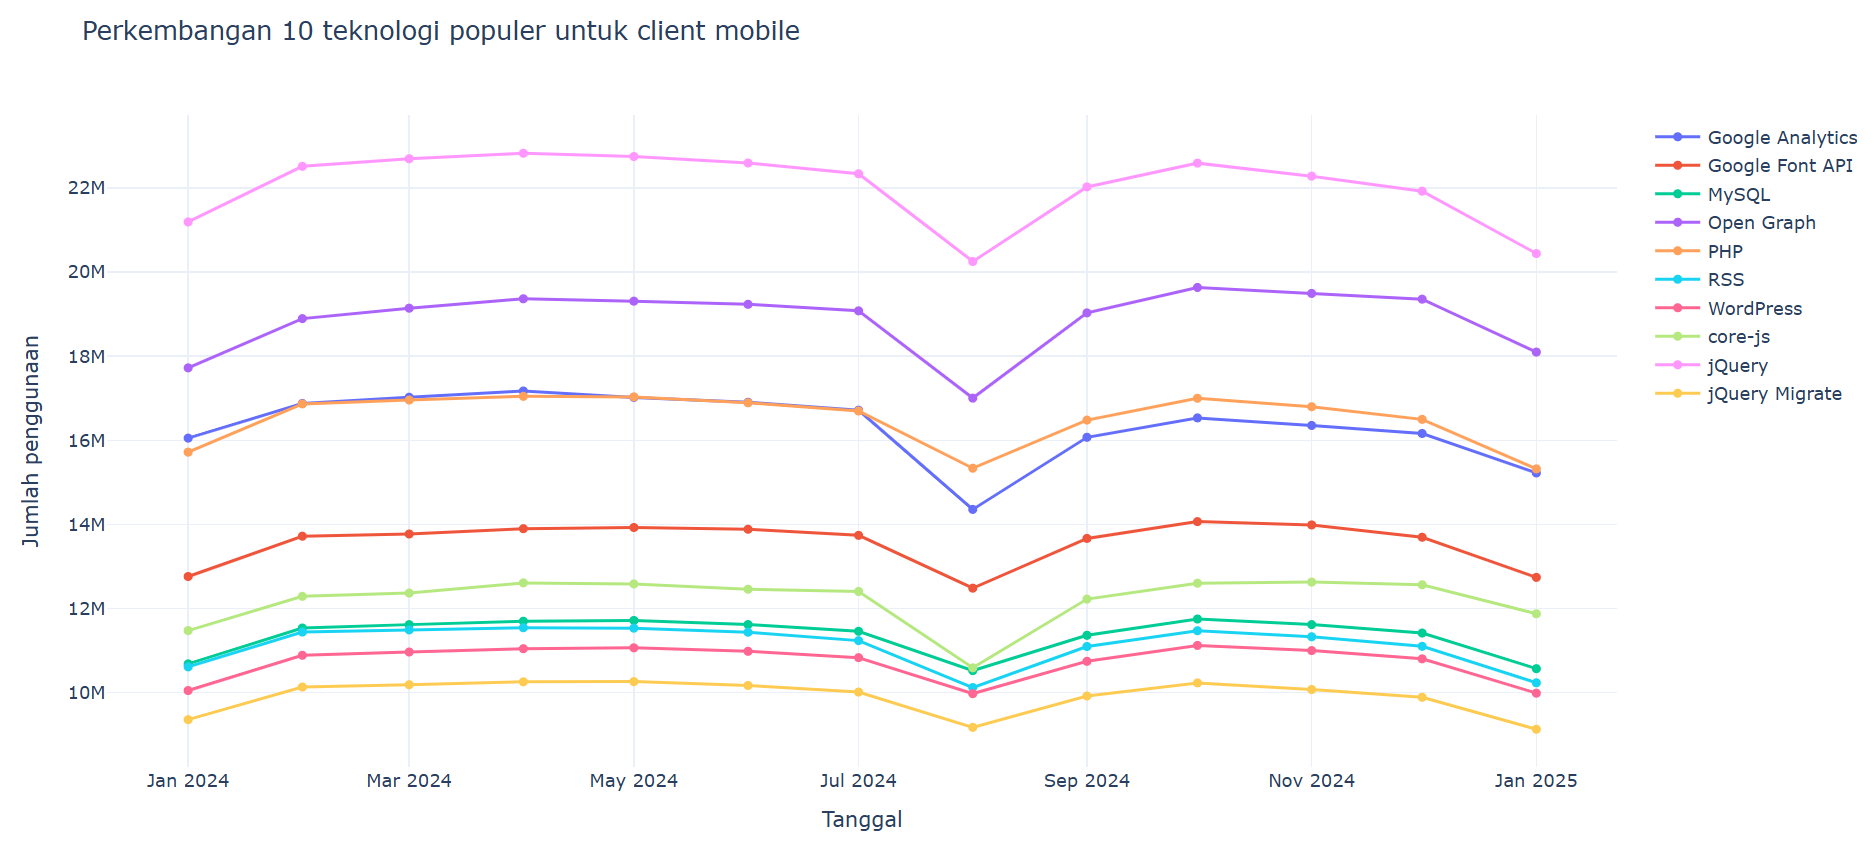
\includegraphics[width=0.7\linewidth]{Gambar/perkembangan 10 teknologi mobile.png}
    \caption{Perkembangan sepuluh teknologi populer pada \textit{client} \mobile}
    \label{fig:10mobile}
\end{figure}

Hasil visualisasi untuk data berdasarkan persentasepenggunaan dapat dilihat pada Gambar~\ref{fig:persentmobile}. Hasilnya menunjukan untuk semua teknologi adanya kenaikan persentase penggunaan pada bulan Agustus 2024. Hal ini dikarenakan total jumlah penggunaan teknologi pembuatan \web di bulan tersebut merupakan yang paling kecil.

\begin{figure}
    \centering
    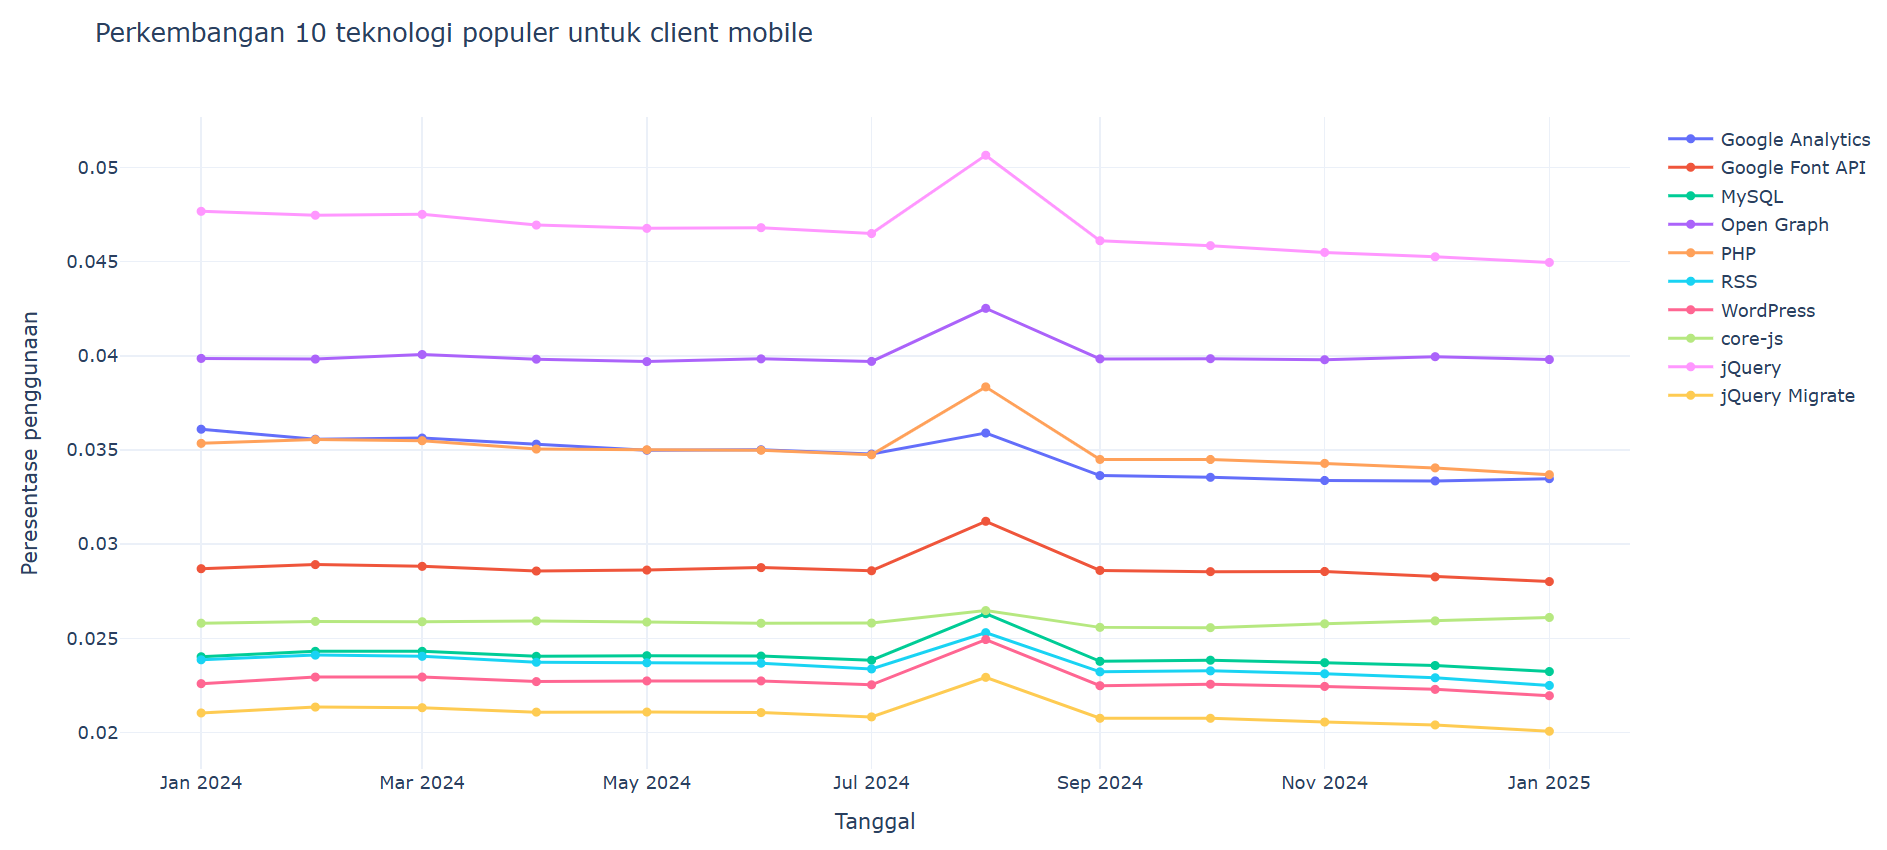
\includegraphics[width=0.7\linewidth]{Gambar/perkembangan persentase mobile.png}
    \caption{Perkembangan persentase penggunaan sepuluh teknologi populer pada \textit{client} \mobile}
    \label{fig:persentmobile}
\end{figure}

\subsubsection{Perkembangan Sepuluh Teknologi pada \textit{Client} \desktop}

Metode yang dilakukan untuk melihat perkembangan sepuluh teknologi yang paling banyak digunakan untuk \textit{client} \desktop sama seperti pada Bagian~\ref{subsub:10mobile} yaitu memisahkan data yang memiliki \textit{client} \desktop terlebih dahulu kemudian melakukan pengolahan sehingga mendapatkan hasil visualisasi yang diinginkan. Visualisasi yang dilakukan didasarkan pada dua hal yaitu jumlah penggunaan teknologi dan persentase penggunaan teknologi. Hasil visualisasi berdasarkan jumlah penggunaan nya dapat dilihat pada Gambar~\ref{fig:10dekstop}. Pada \textit{client} \desktop penggunaan teknologi PHP tidak sebanyak pada perangkat \mobile. Kemudian pada tanggal 1 Agustus 2024 juga semua teknologi mengalami penurunan penggunaan. Namun untuk \textit{client} \desktop penggunaan semua teknologi tidak langsung mengalami kenaikan di bulan september namun baru meningkat kembali di bulan Oktober.
\begin{figure}[H]
    \centering
    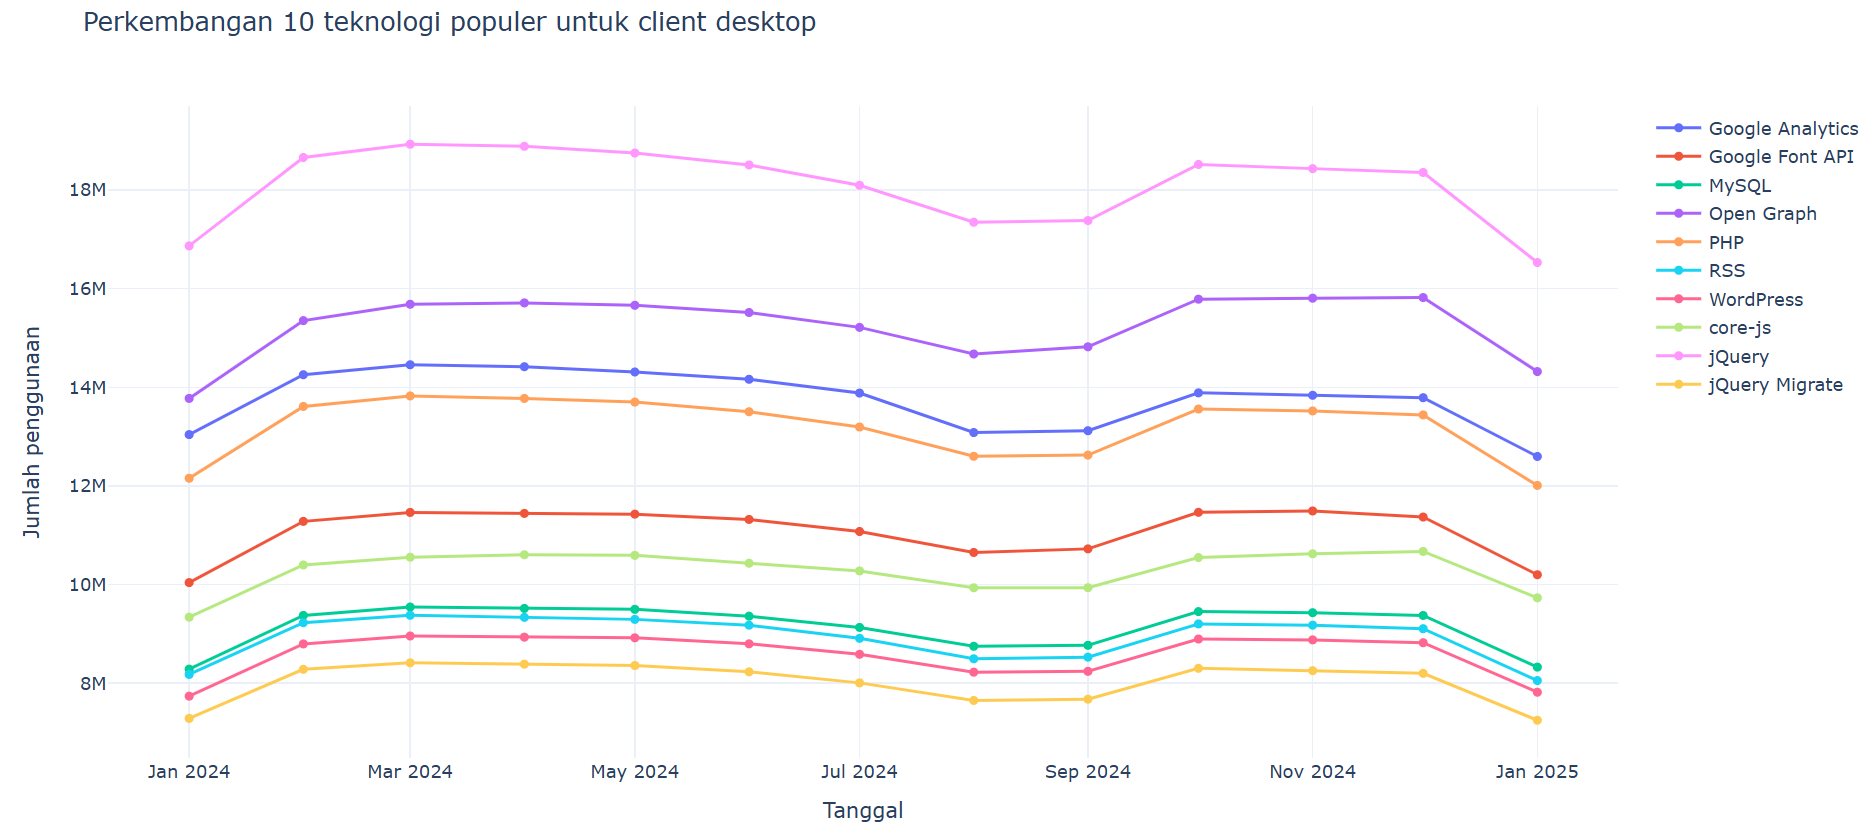
\includegraphics[width=0.7\linewidth]{Gambar/Perkembangan 10 teknologi pada desktop.png}
    \caption{Perkembangan sepuluh teknologi yang populer untuk \textit{client} \desktop}
    \label{fig:10dekstop}
\end{figure}

Hasil visualisasi untuk persentase penggunaan pada \textit{client} \desktop dapat dilihat pada Gambar~\ref{fig:persentasedesktop}. Hasil nya menunjukan bahwa adanya kenaikan persentase penggunaan teknologi popule pada bulan Agustus 2024. Hal ini dikarenakan jumlah penggunaan total pada bulan Agustus nilai nya paling rendah dibandingkan dengan bulan yang lain sehingga persentase untuk semua teknologi akan naik.
\begin{figure}[H]
    \centering
    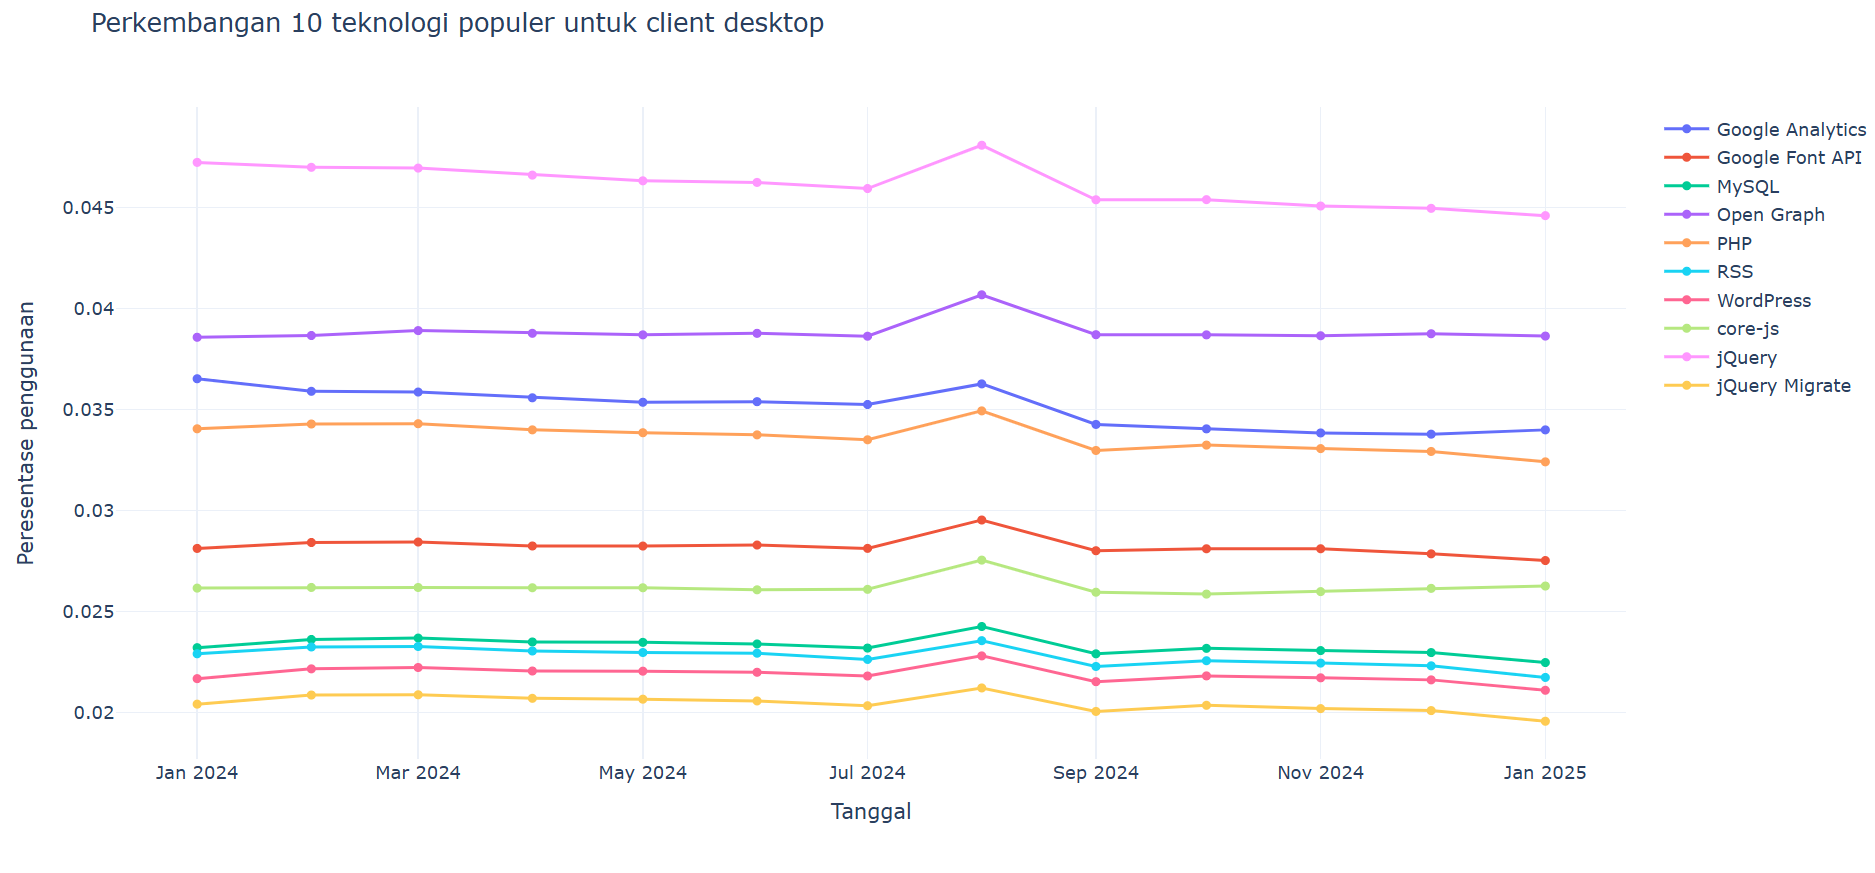
\includegraphics[width=0.7\linewidth]{Gambar/Perkembangan persentase pada desktop.png}
    \caption{Perkembangan persentase penggunaan sepuluh teknologi populer pada \textit{client} \desktop}
    \label{fig:persentasedesktop}
\end{figure}

\section{Eksplorasi \textit{Library Python}}
\label{sec:library}

\subsection{\textit{Tkinter}}
\label{subsec:tkinter}

\textit{Library} ini digunakan untuk membuat tampilan antarmuka grafis yang menggunakan Tcl/Tk sebagai dasarnya seperti yang sudah dijelaskan dalam \ref{sec:tkinter}. Ada beberapa hal yang dapat dilakukan dengan menggunakan library ini seperti contohnya membuat tampilan grafis untuk menampilkan grafik perkembangan teknologi pembuatan \web.

Tampilan yang dapat dibuat tentunya harus memiliki fitur yang dapat digunakan oleh pengguna nantinya seperti pengguna dapat memilih teknologi yang ingin dilihat perkembangannya, pengguna dapat memilih rentang waktu untuk melihat perkembangan teknologinya, dan pengguna juga dapat melihat perkembangan teknologi berdasarkan jumlah penggunaannya atau persentase penggunaannya. Hal ini dapat dicapai dengan beberapa cara. Untuk pemilihan teknologi, pengguna dapat memilih satu atau lebih teknologi yang ingin dilihat. 

\textit{Tkinter} memiliki beberapa cara untuk memenuhi kebutuhan-kebutuhan yang sudah disebutkan, misalnya untuk memilih teknologi yang ingin dilihat perkembangannya dapat digunakan \textit{checkbox}. Kode~\ref{kode:checkbox} adalah kode yang digunakan agar dapat menampilkan \textit{checkbox} yang berisi teknologi yang ingin dilihat perkembangannya.

\begin{lstlisting}[language=Python, caption=Kode untuk menampilkan \textit{checkbox} berisi teknologi, label=kode:checkbox]

     self.checkbox_frame = ttk.Frame(root)
     self.checkbox_frame.pack()

        self.tech_vars = {}
        for tech in df.columns:
            var = tk.BooleanVar(value=False)
            cb = ttk.Checkbutton(self.checkbox_frame, text=tech, variable=var)
            cb.pack(anchor='w')
            self.tech_vars[tech] = var
    
\end{lstlisting}

Kode \verb|self.checkbox_frame = ttk.Frame(root)| adalah kode untuk membuat \textit{frame} yang akan menjadi wadah bagi sekumpulan \textit{checkbox} tersebut. Parameternya diisikan \verb|root| karena \textit{frame} ini merupakan \textit{child widget} dari \textit{widget} \verb|root|, seperti yang sudah dijelaskan pada Bagian~\ref{sec:tkinter}. Baris kode \verb|self.checkbox_frame.pack()| berguna untuk meletakkan widget \textit{frame} di dalam jendela tampilan secara otomatis, dalam kata lain baris kode ini berperan sebagai \textit{geometry manager}. Baris selanjutnya adalah pengulangan yang dilakukan untuk memasukkan teknologi ke dalam \textit{checkbox}. Hasil dari menjalankan Kode~\ref{kode:checkbox} dapat dilihat pada Gambar~\ref{fig:checkbox}

\begin{figure} [H]
    \centering
    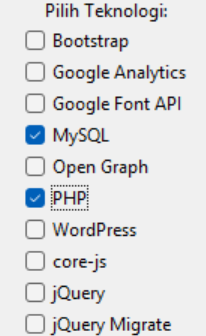
\includegraphics[width=0.25\linewidth]{Gambar/checkbox.png}
    \caption{Checkbox yang berisi teknologi yang dapat dipilih untuk dilihat perkembangannya}
    \label{fig:checkbox}
\end{figure}

Selain memilih teknologi yang ingin dilihat, pengguna juga dapat memilih rentang waktu yang ingin dilihat perkembangannya. Salah satu yang dapat digunakan adalah dengan menggunakan \textit{text box}. Kode~\ref{kode:tanggal} dapat dijalankan untuk memenuhi kebutuhan ini.

\begin{lstlisting}[language=Python, caption=Kode untuk menampilkan \textit{textbox} berisi tanggal, label=kode:textbox]

         ttk.Label(frame, text="Dari (YYYY-MM):").grid(row=0, column=0)
        self.start_var = tk.StringVar(value=df.index[0])
        self.start_entry = ttk.Entry(frame, textvariable=self.start_var, width=10)
        self.start_entry.grid(row=0, column=1)
    
\end{lstlisting}

Baris kode \verb|self.start_var = tk.StringVar(value=df.index[0])| berguna untuk mengisi \textit{textbox} dengan tanggal pertama yang ada di dalam data yang dimiliki yang kemudian diubah ke dalam bentuk \textit{string}. Baris kode \verb|self.start_entry = ttk.Entry(frame, textvariable=self.start_var, width=10)| berguna untuk membuat \textit{textbox} untuk memilih tanggalnya. Parameter \verb|frame| digunakan karena \textit{textbox} ini adalah \textit{child widget} dari \textit{widget frame}. Baris kode \verb|self.start_entry.grid(row=0, column=1)| berperan sebagai \textit{geometry manager} yang akan menempatkan \textit{textbox} pada baris 0 dan kolom 1 pada \textit{widget frame}. Hasil yang didapat setalah menjalankan kode~\ref{kode:textbox} dapat dilihat pada Gambar~\ref{fig:textbox}

\begin{figure}[H]
    \centering
    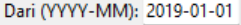
\includegraphics[width=0.25\linewidth]{Gambar/textbox.png}
    \caption{\textit{Textbox} untuk memilih tanggal mulai rentang waktu untuk melihat perkembangan teknologi}
    \label{fig:textbox}
\end{figure}

Kemudian pengguna juga dapat memilih perkembangan yang ingin dilihat berdasarkan jumlah penggunaan atau persentase penggunaan teknologi. Untuk memenuhi hal tersebut maka salah satu caranya adalah dengan menggunakan \textit{radio buton}. Kode~\ref{kode:radio} adalah kode yang dapat digunakan untuk membuat \textit{radio button} ini.

\begin{lstlisting}[language=Python, caption=Kode untuk menampilkan \textit{radio button} untuk memilih grafik yang dilihat, label=kode:radio]

        self.mode_var = tk.StringVar(value="jumlah")
        rb1 = ttk.Radiobutton(mode_frame, text="Jumlah Penggunaan", variable=self.mode_var, value="jumlah")
        rb2 = ttk.Radiobutton(mode_frame, text="Persentase", variable=self.mode_var, value="persentase")
        rb1.pack(anchor='w')
        rb2.pack(anchor='w')
    
\end{lstlisting}

Baris kode \verb| self.mode_var = tk.StringVar(value="jumlah")| merupakan variabel yang menyimpan mode yang akan dipakai. Kode \verb|rb1 = ttk.Radiobutton(mode_frame, text="Jumlah Penggunaan", variable=self.mode_var, value="jumlah")| berguna untuk membuat \textit{radio button} yang membuat grafik yang dilihat merupakan grafik berdasarkan jumlah penggunaan. Kode \verb| rb1.pack(anchor='w')| berguna untuk menempatkan \textit{radio button} pada jendela tampilan secara otomatis. Hasil dari kode~\ref{kode:radio} dapat dilihat pada Gambar~\ref{fig:radio}

\begin{figure}[H]
    \centering
    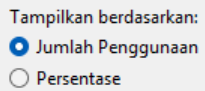
\includegraphics[width=0.25\linewidth]{Gambar/radio.png}
    \caption{\textit{Radio button} untuk memilih mode grafik yang ingin ditampilkan}
    \label{fig:radio}
\end{figure}

Hasil secara utuh dapat dilihat pada Gambar~\ref{fig:guiutuh}. Terlihat adanya tombol ``Tampilkan Grafik'' yang akan mengarahkan pengguna ke \textit{browser} untuk melihat grafik perkembangan teknologi yang sudah dipilih.

\begin{figure}[H]
    \centering
    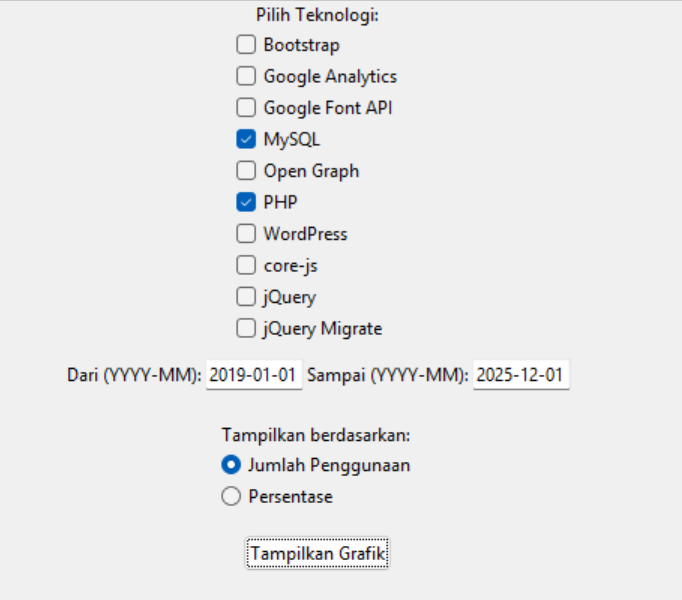
\includegraphics[width=0.25\linewidth]{Gambar/Guiutuh.png}
    \caption{Tampilan \textit{GUI} untuk melihat perkembangan teknologi pembuatan \web}
    \label{fig:guiutuh}
\end{figure}